\documentclass[9pt,twocolumn,twoside]{gsajnl}
% Use the documentclass option 'lineno' to view line numbers

\articletype{inv} % article type
% {inv} Investigation 
% {gs} Genomic Selection
% {goi} Genetics of Immunity 
% {gos} Genetics of Sex 
% {mp} Multiparental Populations

\title{TCGA RNA-seq data analysis in breast invasive carcinoma}

\author[$\ast$]{Garcia-Serrano, A}
\author[$\ast$,1]{Gilabert-Navarro, JF.}
\author[$\ast$]{Madsen-Choppi, LPN.}

\affil[$\ast$]{Universitat Pompeu Fabra}

\keywords{Breast Invasive Carcinoma; RNA-seq; TCGA Project; Bioinformatics; Differential Expression; Functional Enrichment}

\runningtitle{TCGA RNA-seq data analysis in breast invasive carcinoma} % For use in the footer 

\correspondingauthor{Gilabert-Navarro, JF.}

\begin{abstract}
Breast cancer is the most common malignant cancer affecting
women and is the second leading cause of cancer death world-
wide. In this work, we have analyzed data from RNA-seq experiments provided by the TGCA. We have analyzed the differential expression of many genes between tumoral samples and non-tumoral samples, both obtained from the same individual, using a paired design. Using this model, we found about 10200 genes significantly differentially expressed deppending of the type of tissue. Finally, we performed a functional enrichment analysis with Gene Ontology (Biological Process) in order to see the pathways affected by these differentially expressed genes. In this way, we observed the inflammatory and metabolic processes as the main differentially expressed pathways in breast cancer.
\end{abstract}

\setboolean{displaycopyright}{true}

\begin{document}

\maketitle
\thispagestyle{firststyle}
\marginmark
\firstpagefootnote
\correspondingauthoraffiliation{JF Gilabert: joanfrancesc.gilabert01@estudiant.upf.edu}
\vspace{-11pt}%

\section*{Introduction}
Breast cancer is the most common malignant cancer affecting women and is the second leading cause of cancer death worldwide\citep{rosam}. This disease has more than 1,300,000 cases and 450,000 death each year around the world\citep{cangen}.
This disease is widely heterogeneous, having a large and diverse set of molecular, histological and clinical behaviours depending of the tumour\citep{rosam}. In addition, the response to specific treatments it is also very different between patients. For this reason, breast cancer was been classified in different subtypes in order to achieve a better understanding of these disease. Traditionally, the classification has been based on clinicopathological features such as tumor type and size, lymph node status and histological grade\citep{rosam}. Actually, nowadays this disease is an entity difficult to classify due to the wide range of classifiers that we can take into account: histological, immunopathological, transcriptional, genomic, miRNA-based, epigenetic, microenvironmental, macroenvironmental, longitudinal and other classifiers\citep{breast}. However, we have an actual classification based on simple molecular characteristics\citep{cangen}
\begin{itemize}
\item \textbf{Estrogen receptor (ER) positive:} The most numerous and diverse, with several genomic tests to assist in predicting outcomes for ER+ patients receiving endocrine therapy.
\item \textbf{ HER2 or ERBB2 amplified:} Great clinical success because of effective therapeutic targeting of HER2, which has led to intense efforts to characterize other DNA copy number aberrations.
\item \textbf{Triple negative:} Lacking expression of ER, progesterone receptor (PR) and HER2. It is also known as basal-like breast cancers, are a group with only chemotherapy options, and have an increased incidence in patients with germline BRCA1 mutations or of African ancestry.
\end{itemize}

The more frequently mutated genes in breast cancer are BRCA1, BRCA2, PALB2, ATM, TP53, PTEN, PIK3CA, AKT1, GATA3, CDH1, RB1, MLL3, MAP3K1, CDKN1B, between others\citep{acs}. If we focus in their functionalities, these genes are linked with DNA repair, control of cell cycle, apoptosis, cell proliferation and gorwth. BRCA1 and BRCA2 mutations are the most common cause of hereditary breast cancer\citep{acs}. In addition, women with these mutations also have higher risk of developing other cancers, mainly ovarian cancer\citep{acs}. In case of BRCA1 mutations, the risk compared with the population is about 60\% meanwhile in BRCA2 mutations is about 45\%\citep{acs}. 
\vspace{2 mm}

Anyway, as we describe above, each tumour has a high specific profile with a lot of different variables difficulting the establishment of simple classifiers. In the last decades, molecular knowledge advances have allowed to initialize personalized medicine. In this way, we can use targeted drugs to very specific tumour types with a high percentage of effectiveness. The main problem of this personalized medicine is the very reduced number of tumours in which we can observe a remission. This is due to the very high specificity of the treatments, useful only for a tumour with a concrete molecular characteristics. 

\vspace{2 mm}

In this way, new technologies focused not only in mRNA expression profiling, DNA copy number analysis and massively parallel sequencing but also in detecting abnormalities in DNA methylation, miRNA and protein expression provides a wider range of information\citep{cangen}. Therefore, we can use all these tools in order to get a deeper understanding about tumor molecular mechanisms resulting in advances towards personalized medicine.

\section*{Materials and Methods}
All the following analysis were performed with \verb+R Studio Software Version 0.99.489 (R version 3.3.0)+. In this work we have used the following R packages: $SummarizedExperiment$, $edgeR$, $geneplotter$, $sva$, $limma$, $GOstats$, $org.Hs.eg.db$ and $xtable$.

\subsection*{Data Availability}
\vspace{2 mm}

Our RNA-seq data set was obtained from The Cancer Genome Atlas (TCGA) Project. The data sets of this Project are tables of RNA-seq counts generated by Rahman et al \citep{Rahman15112015} from the TCGA raw sequence read data using the $Rsubread / featureCounts$ pipeline for all data sets.
\vspace{2 mm}

We chose Breast Invasive Carcinoma RDS file in order to perform our analyses. This set is composed by 1119 tumoral tissue samples and 113 healthy tissue samples. In this work we focus in a particular subset. The subsetting criteria was the selection of paired data; we only used those samples which have both tumoral and healthy tissue from the same patient. In this way, we tried to minimize the effect of inter-personal variability due to the differences in genetic background.
\vspace{2 mm}
  
So, first of all we filtered our data by the common \verb+brc_patient_barcode+ and replace our original data by this subset containing 212 samples in total; 106 tumoral tissue samples and 106 healthy tissue samples. All the statistical analysis explained below were performed using this new data set.


\subsection*{Statistical Analysis} 
\vspace{2mm}

\textbf{Quality assessment}
\vspace{2mm}

Before starting with the differential expression analysis we need to ensure the quality of our data in order to avoid bias in our results and in consequence, the extraction of wrong conclusions. 
\vspace{2mm}

Expression levels were considered taking into account the $log_{2}$ of $CPM$ values of expression. The first analyses that we performed were observe gene expression distribution and filtering again by genes less expressed. We considered a cutoff of 1 $log CPM$ unit as a minimum value of expression to select genes being expressed across samples.
\vspace{2mm}

After that, we calculated the normalization factors on this new filtered data set using the TMM method implemented in the edgeR package and we generated the MA-plots both for normal and tumoral samples (see in $Supplementary Material$).
\vspace{2mm}

Batch effect identification tests were performed taking into account different elements of the TGCA barcode such as tissue source site, the center where the samples were processed, the plate, the sample vial and the portion analyte (molecular specimen extracted; total RNA or whole genome amplified for example). After considering the variables described above, we performed the tests related with the hierarchical clustering and multidimensional scaling examining the samples by the tissue source site (TSS). In this part we used again $log CPM$ values with a higher prior count to moderate extreme fold-changes produced by low counts. Finally, we generated a dendogram of hierarchical clustering of samples by TSS (see on $Results$ section). 
\vspace{2mm}

\textbf{Differential expression analysis}
\vspace{2mm}

In this section we want to analyze how many genes are differentially expressed (DE) across normal and tumoral samples. In order to do that, we need to create a model to start analyzing our data set. We have created two models, a simple model that only considers the type of sample (tumor or not) and one that also takes into account the patient barcode. It is important to introduce this variable into our model because of we want to avoid bias produced by variability in genetic background across individuals. The models were implemented following the pipeline of the limma package. After creating the model and before the statistics, we used the surrogate variable analysis (SVA) to account for unknown covariates. Finally, visualized our DE results with a volcano plot (see also in $Results$ section).
\vspace{4mm}

\textbf{Functional enrichment analysis}
\vspace{2mm}

The last part of our analysis is aimed at the functional interpretation of our DE genes results. To do that, we focused on the Gene Ontology biological processes since we are interested in understanding which pathways are more affected across breast tumors. To perform this analysis we used the packages $GOstats$ to obtain the information relative to Gene Ontology and link it with our RNA-seq data, $org.Hs.eg.db$ to obtain the genome wide annotation for Homo Sapiens using Entrez Gene Identifiers and finally we use $xtable$ to generate the output results. First step was to extract the differential expressed genes (p-value < 0.05) obtained previously, later we defined the gene universe with all the Entrez IDs of genes contained in our data. With these data we run the hypergeometric tests for GO association, using a conditional analysis.
\vspace{2mm}

Finally we filtered the results only considering GO terms with gene size and gene counts greater than 5, since those with size smaller than 5 are not so reliable. To finish with this part the final results were ordered by the Odds Ratio and exported into an html output for a better visualization (view in $Results$ section, more specific information is available in $Supplementary Material$).

\section*{Results and Discussion}
\subsection*{Quality assesment} 
\vspace{1mm}

Distribution of expression levels among genes were quite similar both in tumor and normal samples ($Supplementary Material$). Concerning the filtering of low - expressed genes, we masked those which $log CPM$ were lower or equal than 1. This step filtered out 8260 genes, from 20115 at the beginning to 11855 genes after filtering.

MA-plots showed that profiles of tumor samples and normal ones didn't show strong differences in expression - levels (MA-plots available in $Supplementary Material$).
\vspace{1mm}

Regarding the search of potential surrogate of Batch effect indicators, we analyzed the distribution of samples among the following variables: tissue source site, center, plate, portion analyte and sample vial We observed that all samples were sequenced at the same center. In addition, all samples belong to one of two combinations of tissue type and vial, matching the expected tumor and normal distribution. The only variable that can be, potentially, a Batch effect indicator was the tissue source site. After analyzing the hierarchial clustering of the samples (see figures S6 and S7 in $Supplementary Material$), we can observe that samples cluster primarily by sample type (tumor - normal). Therefore, no batch effects were observed related to clustering linked to TSS. We continued the analysis without removing any sample.
\vspace{2mm}

\subsection*{Differential Expression Analysis} 
\vspace{2mm}

We analyzed the number of surrogate variables (SV) for our model including both type of sample and patient barcode. The number of significant SVs were 14, so taking them into account, the linear model showed us that, only focusing in sample type, we have 4811 genes underexpressed and 5396 overexpressed in tumors vs healthy tissue. In addition, we have obtained a long list of over/underexpressed genes for each patient (106 patients in total, see in $Supplementary Material$).
\vspace{2mm}

p-value distributions and qqplots of both models created yielded similar results. We observed an approximately uniform p-value distribution of the non-significant p-values and a marked high frequency for the significant ones. In addition, the slope of the qqplots is much higher than 1 (more information in $Supplementary Material$). 
\vspace{2mm}

To compare the two models, we created volcano plots for both of them (Figure \ref{fig:spectrum}). The shape of the volcano plots are very similar, with some differences in the highlighted genes. Quantitatively, the second model (type of sample + patient barcode) yields about 700 more DE genes (see $Supplementary Material$ for further details), thus we see how the more complex model increases our statistical power. Finally, we consider 10200 genes significantly differentially expressed with a p-value < 0.05 and FDR of 10\%.

\begin{figure}[htbp]
\centering
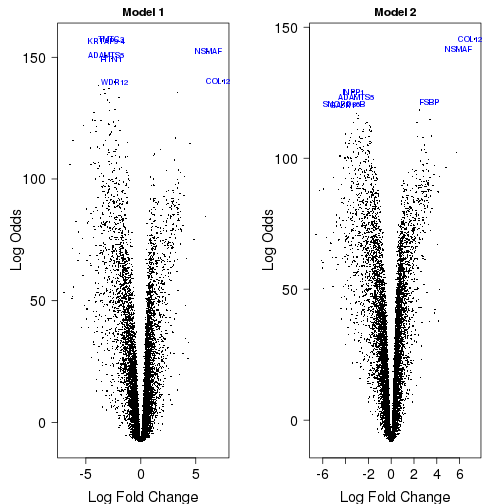
\includegraphics[width=70mm]{volcanotex-1}
\caption{Comparison of the volcano plots for the two models created. Model 1 only takes into account the type of sample (normal/tumor) and Model 2 takes also into account the paired samples (patient barcode).}%
\label{fig:spectrum}
\end{figure}

\subsection*{Functional Enrichment Analysis} 
\vspace{2mm}

In this section we only 
consider GO terms with gene size and gene counts greater than 5 in order to obtain more reliable results. An html file was generated containing all the detailed results ordered by Odds Ratio (See in $Supplementary Material$).
\vspace{2mm}

Before starting to analyze the main results obtained, it is important to take into account that these are the GO terms differentially expressed, but we don't know if these pathways are over-activated or repressed by this genetic differential expression. In addition, the genes inside each GO term could be over-expressed or under-expressed. Another important fact is that not all the genes implicated in one pathway have the same repercussions in it, some of them will help to the activation and other could inhibit the processes implicated. 
\vspace{2mm}

The results are summarized in Table \ref{table}. In the table, we can observe that the pathway with the highest Odds Ratio (Inf, not shown in Table \ref{table} for brevity, a fully detailed table is available in the $Suplementary Material$) and lowest p-value (0.0, theoretical) is the regulation of acute inflammatory response. In addition, the 4th position of the top 10 GO Terms it is also related with inflammation. This results are concordant with the scientific evidence that links inflammatory processes with the tumor development. It is well known how the inflammatory processes are risk factors in breast cancer by modulation of progression and implying a less response to treatment \citep{Murray01022015}. But not all inflammatory components have the same effect in tumour tissue. We know that there are components such as some interleukins and some cytokines that improves tumour progression and development \citep{Esquivel-Velzquez2014}. In contraposition, other components such as tumor necrosis factors or some cytokines improves the protection against breast cancer \citep{Esquivel-Velzquez2014}. In this way, we could observe how the components of the same pathway could be dual roles in breast cancer. 
\vspace{2mm}

In addition, it is important also to reflect how inflammation is not an isolate and related process. This inflammatory implication could be produced by obesity, since it is estimated that the number of cancer cases caused by obesity are around 20\% \citep{DePergola2013,BaumgartenFrasor}. Severe overweight could lead to systemic inflammation that could provide proliferative advantages in tumor tissue \citep{Iyengar2013}.
\vspace{2mm}

Another important perturbation produced by obesity is done in metabolic pathways. Recent studies show relationship between cancer, obesity, type II diabetes and oxidative stress \citep{Ferroni2015,Flanagan2015} making our GO results stronger, since superoxide metabolic process and glucuronate metabolic process are between our top 10 enriched GO terms.
\vspace{2mm}

It is well known that metabolism of tumoral cells is clearly different than the metabolism in the equivalent healthy cells. Glucose, lactate, pyruvate, hydroxybutarte, acetate, glutamine and fatty acids metabolism rates are considerably heightened in tumors \citep{Martinez-Outschoorn2016}. This higher ATP generation as an energy source provide tumoral cells advantages to improve the proliferation and progression rates.
\vspace{2mm}

Sodium ion homeostasis is also a remarkable GO term result since it is the second in the top 10 enrichment (Table \ref{table}) with a p-value of 0.01. This pathway was related previously with several malignant tumors such as Glioblastoma multiforme, hepatocellular carcinoma, lung cancer and, in our interest type, breast cancer \citep{DaminCong2015}. Ion transporters are important in homeostasis, cell volume and cellular signal transduction, processes frequently affected in tumours. In addition, sodium transport controls pH gradient, which is also an important differential factor in tumoral cells. There is some evidence about the cytoplasmic alkalinization in breast cancer by an increased sodium channels activity, fact that turn this tumors more metastasic \citep{Amith1259,Fraser20130105}. Moreover, metastasis and malignancy are favored by angiogenesis processes. This is clearly represented also in our GO terms Table \ref{table} by cellular response to vascular endothelial growth factor stimulus.
\vspace{2mm}

This signal transduction often affects DNA/nucleus regulation processes. This fact is in agreement with our results, since protein import into nucleus (translocation) and negative regulation of DNA replication are GO terms in our top 10 enriched items. As we know, tumoral cells have increased proliferative rates (in most cases), so in this way, regulation of DNA replication is clearly a process that would be affected.
\vspace{2mm}

Finally, we have two more enriched GO terms less obvious at first glance: endochondrial bone morphogenesis and adult walking behaviour. Regarding bone morphogenesis pathways, the alteration of the related genes could lead to a metastasis tendency in tumoral cells. Besides, this bone marrow alteration could be due to the chemotherapy applied on tumors, being a cause and not a consequence of this differential expression. On the other hand, adult walking behaviour could be related with the existing link between breast cancer and lifestyle. As we comment at the beginning of this section, obesity is a known risk factor in cancer. Moreover, we know that exercise and diet restriction are protective factors against this disease  \citep{Chlebowski}. At this point, we could think that this GO term result could be linked with the other ones since physical activity modules the previous explained processes: metabolic rates, inflammation and immune function between others \citep{McTiernan2008}.
\vspace{2mm}

To conclude this part, we could say that our top 10 enriched GO terms are concordant with the literature and the previous knowledge. In addition, this results help us understand how all the processes in health and disease physiology are strongly linked and are not independent and isolated pathways.


\begin{table}[ht]
\centering
\caption{\bf Top 10 enriched GO Terms. Odds Ratio values are not shown since all of them are "Inf".}
\begin{tableminipage}{\textwidth}
\begin{tabular}{cccp{3cm}}
  \hline
 Pvalue & Count & Size & Term\\ 
  \hline
0.00 &  36 &  36 & regulation of acute inflammatory response\\ 
0.01 &  32 &  32 & sodium ion homeostasis \\ 
0.02 &  28 &  28 & protein import into nucleus, translocation\\ 
0.02 &  27 &  27 & regulation of humoral immune response\\ 
0.02 &  26 &  26 & superoxide metabolic process \\ 
0.02&  26 &  26 & cellular response to vascular endothelial growth factor stimulus\\ 
0.02 &  25 &  25 & endochondral bone morphogenesis\\ 
0.03 &  23 &  23 & negative regulation of DNA replication\\ 
0.03 &  23 &  23 & glucuronate metabolic process\\ 
0.04 &  22 &  22 & adult walking behavior\\ 
   \hline
\end{tabular}
\end{tableminipage}
\label{table}
\end{table}

\section*{Conclusions}
With all our analysis we could conclude that the main processes affected in breast invasive carcinoma are related with inflammation, metabolism, nucleus-DNA regulation processes, oxidative stress and angio/vasculogenesis (among others). We observed pathways previously related in other studies with this and other types of cancer. Our results are in agreement with the actual scientific evidence and provide a bioinformatics tool approach in order to manage, extract and select relevant information in a fast way of high-troughput sequencing technologies.
\vspace{2mm}

It is also important to consider how all these pathways are linked and how the molecules involved interact between them, in order to be able to use this information to advance towards personalized medicine focused in the molecular characteristics of each specific tumor. It is necessary to consider all the pathways as little fractions of a complete interconnected system. Any progress in cancer treatment will come of a better understanding of the molecular details and, at the same time, the holistic point of view that considers our organism as a complex system that integrates many functionalities.

\section*{Acknowledgments}
We wish to thank Universitat Pompeu Fabra and Dr. Robert Castelo for the lessons imparted and the help provided to manage all this data. We are grateful also with TCGA Project, which provided the data analyzed in this work.

\bibliography{biblio.bib}

\end{document}